\documentclass{article}
\usepackage[utf8]{inputenc}
\usepackage{graphicx}
\usepackage{whilecode2}

\title{Practica 4}
\author{Jose Antonio Guardeño Algar}
\date{December 2022}

\begin{document}

\maketitle
\section{Ejercicio 1}
\maketitle
1. Create the simplest WHILE program that computes the diverge function (with zero arguments) and compute the codification of its code.
\newline
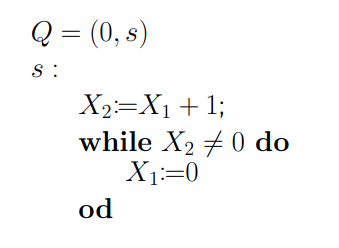
\includegraphics[width=6cm]{imagen_2022-12-26_164453139.png}
\newline
El cual es CODE2N("X2:=X1+1; while X2!=0 do X1:=0 od")
ans = 10876
\maketitle
\section{Ejercicio 2}
\maketitle
\newline
2. Create an Octave script that enumerates all the vectors.
\newline
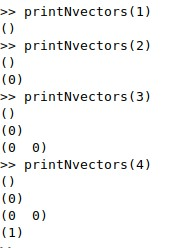
\includegraphics{praactica42.jpg}
\newline
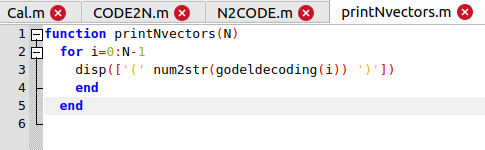
\includegraphics{imagen_2022-12-26_173832950.png}
\section{Ejercicio 3}
\maketitle
3. Create an Octave script that enumerates all the WHILE programs.
\newline
Function that represents all the WHILE programs for an index N in Octave.
\begin{verbatim}
function printNwhilePrograms(N)
for i=0:N-1
disp(N2WHILE(i))
end
end
\end{verbatim}
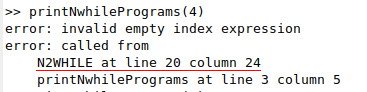
\includegraphics{imagen_2022-12-26_180329923.png}
\end{document}
